\documentclass[tikz,border=5pt,12pt]{standalone}
\usepackage{tikz}

\begin{document}    
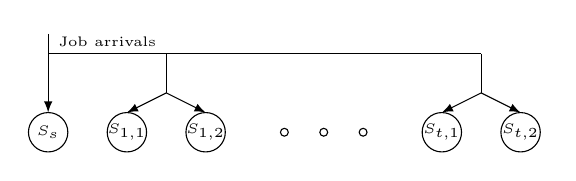
\begin{tikzpicture}[>=latex]

\draw[-] (0,0.25) -- (0,0);
\node at (0.75,0.15) {\tiny Job arrivals};
\draw[->] (0,0) -- +(0,-0.75);
\draw (0,-1) circle [radius=0.25] node {\tiny $S_s$};
\draw[-] (0,0) -- (5.5,0);

\draw[-] (1.5,0) -- (1.5,-0.5);
\draw[->] (1.5,-0.5) -- (1,-0.75);
\draw[->] (1.5,-0.5) -- (2,-0.75);
\draw (1,-1) circle [radius=0.25] node {\tiny $S_{1,1}$};
\draw (2,-1) circle [radius=0.25] node {\tiny $S_{1,2}$};

\draw (3,-1) circle [radius=0.05];
\draw (3.5,-1) circle [radius=0.05];
\draw (4,-1) circle [radius=0.05];

\draw[-] (5.5,0) -- (5.5,-0.5);
\draw[->] (5.5,-0.5) -- (5,-0.75);
\draw[->] (5.5,-0.5) -- (6,-0.75);
\draw (5,-1) circle [radius=0.25] node {\tiny $S_{t,1}$};
\draw (6,-1) circle [radius=0.25] node {\tiny $S_{t,2}$};

\end{tikzpicture}
\end{document}